%# -*- coding: utf-8-unix -*-
%%==================================================
%% thesis.tex
%%==================================================

% 双面打印
%\documentclass[doctor, openright, twoside]{sjtuthesis}
\documentclass[bachelor, openany, oneside, english, submit]{sjtuthesis}

% \documentclass[master, review]{sjtuthesis}
% \documentclass[%
%   bachelor|master|doctor,	% 必选项
%   fontset=fandol|windows|mac|ubuntu|adobe|founder, % 字体选项
%   oneside|twoside,		% 单面打印,双面打印(奇偶页交换页边距,默认)
%   openany|openright, 		% 可以在奇数或者偶数页开新章|只在奇数页开新章(默认)
%   english,			% 启用英文模版
%   review,	 		% 盲审论文,隐去作者姓名、学号、导师姓名、致谢、发表论文和参与的项目
%   submit			% 定稿提交的论文,插入签名扫描版的原创性声明、授权声明 
% ]

% 逐个导入参考文献数据库
\addbibresource{bib/thesis.bib}
% \addbibresource{bib/chap2.bib}

\begin{document}

%% 无编号内容:中英文论文封面、授权页
%# -*- coding: utf-8-unix -*-
\title{深度学习中高校高效学习新样本}
\author{宋肇哲}
\advisor{卢策吾}
% \coadvisor{某某教授}
\defenddate{2014年12月17日}
\school{上海交通大学}
\institute{电子信息与电气工程学院}
\studentnumber{5140309514}
\major{电子信息科学类}

\englishtitle{Efficient Methods for Incremental Learning in Deep Neural Networks}
\englishauthor{\textsc{Zhaozhe Song}}
\englishadvisor{Prof. \textsc{Cewu Lu}}
% \englishcoadvisor{Prof. \textsc{Uom Uom}}
\englishschool{Shanghai Jiao Tong University}
\englishinstitute{\textsc{Depart of XXX, School of XXX} \\
  \textsc{Shanghai Jiao Tong University} \\
  \textsc{Shanghai, P.R.China}}
\englishmajor{A Very Important Major}
\englishdate{Dec. 17th, 2014}


\maketitle

\makeatletter
\ifsjtu@submit\relax
	\includepdf{pdf/original.pdf}
	\cleardoublepage
	\includepdf{pdf/authorization.pdf}
	\cleardoublepage
\else
\ifsjtu@review\relax
% exclude the original claim and authorization
\else
	\makeDeclareOriginal
	\makeDeclareAuthorization
\fi
\fi
\makeatother


\frontmatter 	% 使用罗马数字对前言编号

%% 摘要
\pagestyle{main}
%# -*- coding: utf-8-unix -*-
%%==================================================
%% abstract.tex for SJTU Master Thesis
%%==================================================

\begin{abstract}

在深度学习系统中,数据往往是一步步地采集和增加的。在深度学习领域,一个重要而困难的问题是开发出一套能随着数据的增加而不断提升自己知识的系统。在以往的文献中,这个问题通常被称作增量学习。这样的系统,需要不断地快速地在已有的模型中融合进去新的知识,而不是每次增加了新数据都重新把内部的深度神经网络重新训练一遍,否则开销会很大。在这个工作中,我们利用在物体检测领域经常使用的困难负样本挖掘的方法,提出了一套针对类别不断增加时的增量学习算法。在每次新的类别到来的时候,我们的算法的主循环可以大致分解为以下两步:1)用所数据数据继续训练深度神经网络,并且记录下每个旧类别对神经网络来说最困难的一个图片集合。2)在最困难的图片集合中采样,用它们和新类别的数据再次训练当前的深度神经网络。在第一步中,神经网络模型可以对真实的数据分布进行学习。在第二步中,因为有大量新样本比例,模型被迫快速地学习出新样本的特征,同时又不忘记旧类别中最困难的那些样本,如此往复。我们使用几个典型的深度学习网络结构在图像分类数据集CIFAR-10和CIFAR-100上进行了充分的实验证明我们算法的有效性。我们的方法不仅让模型能快速学习出关于新样本的知识,还能对旧样本维持一个很高的准确率。我们用实验说明我们方法可以始终维持一个较高的平均准确率,而其他底线方法或其他论文中的策略都会让模型很快失败。在CIFAR-100数据集上,我们的算法相比重新训练网络能节省40倍的时间,而仅有$2\%$左右的准确率损失。我们的实验也表明我们的模却是确实可以逐渐学习出越来越好的特征来识别逐渐增长的类别。


\keywords{\large 深度学习 \quad 增量学习 \quad 困难负样本挖掘 \quad 图像分类}
\end{abstract}

\begin{englishabstract}

In deep learning systems, data is usually collected incrementally. A major and tough problem in the field of deep learning is the development of systems that learns incrementally over time from a stream of available data. This problem is typically called incremental learning in literature. Such systems should continuously incorporate new knowledge in a quick manner, without having to re-train the inherent deep neural network every time from scratch. In this work, we proposed an algorithm for class-incremental learning systems, by utilizing hard negative mining techniques that were popular in recent object detection pipelines. Upon the addition of a new class, our main algorithm can be broken down into two steps that are iterated for several times: 1) Further train the deep neural network with all data, and record the hardest examples from every learned class. 2) Sample the hardest images that the model has already learned, and use them, together with the new class of data, to further train the neural network. In the first step, the model learns the data in a true distribution. In the second step, since the majority are new examples, the model is forced to learn features quickly for the new class, but also not forgetting the hardest old examples. We conducted thorough experiments on the image classification datasets CIFAR-10 and CIFAR-100 using representative deep learning structures, and proved the effectiveness of our method. Our method not only enables the model to learn knowledge on the new class very quickly, but is also capable of maintaining high accuracy on the old classes. Our algorithm keeps a high average accuracy our time, while baseline strategies or strategies from other papers fail quickly. In CIFAR-100, our algorithm saves $40\times$ time compared to re-training from scratch when a new class of training images are added, with only about $2\%$ average accuracy loss. Experiments also indicate that our model indeed gradually learns better features to correctly classify more objects. 

\englishkeywords{\large deep learning, incremental learning, hard negative mining, image classification}
\end{englishabstract}



%% 目录、插图目录、表格目录
\tableofcontents
\listoffigures
\addcontentsline{toc}{chapter}{\listfigurename} %将插图目录加入全文目录
\listoftables
\addcontentsline{toc}{chapter}{\listtablename}  %将表格目录加入全文目录
\listofalgorithms
\addcontentsline{toc}{chapter}{\listalgorithmname} %将算法目录加入全文目录

%# -*- coding: utf-8-unix -*-
\begin{nomenclaturename}
\label{chap:symb}

\begin{longtable}{rl}
$\epsilon$     & 介电常数 \\
 $\mu$ 		& 磁导率 \\

\end{longtable}

\end{nomenclaturename}
 % 主要符号、缩略词对照表

\mainmatter	% 使用阿拉伯数字对正文编号

%% 正文内容
\pagestyle{main}
%# -*- coding: utf-8-unix -*-
%%==================================================
%% chapter01.tex for SJTU Master Thesis
%%==================================================

%\bibliographystyle{sjtu2}%[此处用于每章都生产参考文献]
\chapter{Introduction}
\label{chap:intro}
\section{Motivation and Contribution}
In many real world applications, data is collected incrementally. For example, the large-scale image classification dataset ImageNet is becoming larger and larger when more notations become available. For another practical example and also the main origination of this project, imagine a commercial system that can classify merchandise correctly based on the image of the merchandise, as illustrated in Fig.~\ref{fig:merchandise}. It has a large potential to be used by automatic robotic arms used in automatic logistics center or autonomous supermarkets. A robotic arm is shown in Fig.~\ref{fig:arm}. Since there will always be new types of merchandise emerging, this system should always adapt to new merchandise types but also not forgetting the learned merchandise types. Thus in this example, the merchandise data is also incremental.

\begin{figure}[!htp]
	\centering
	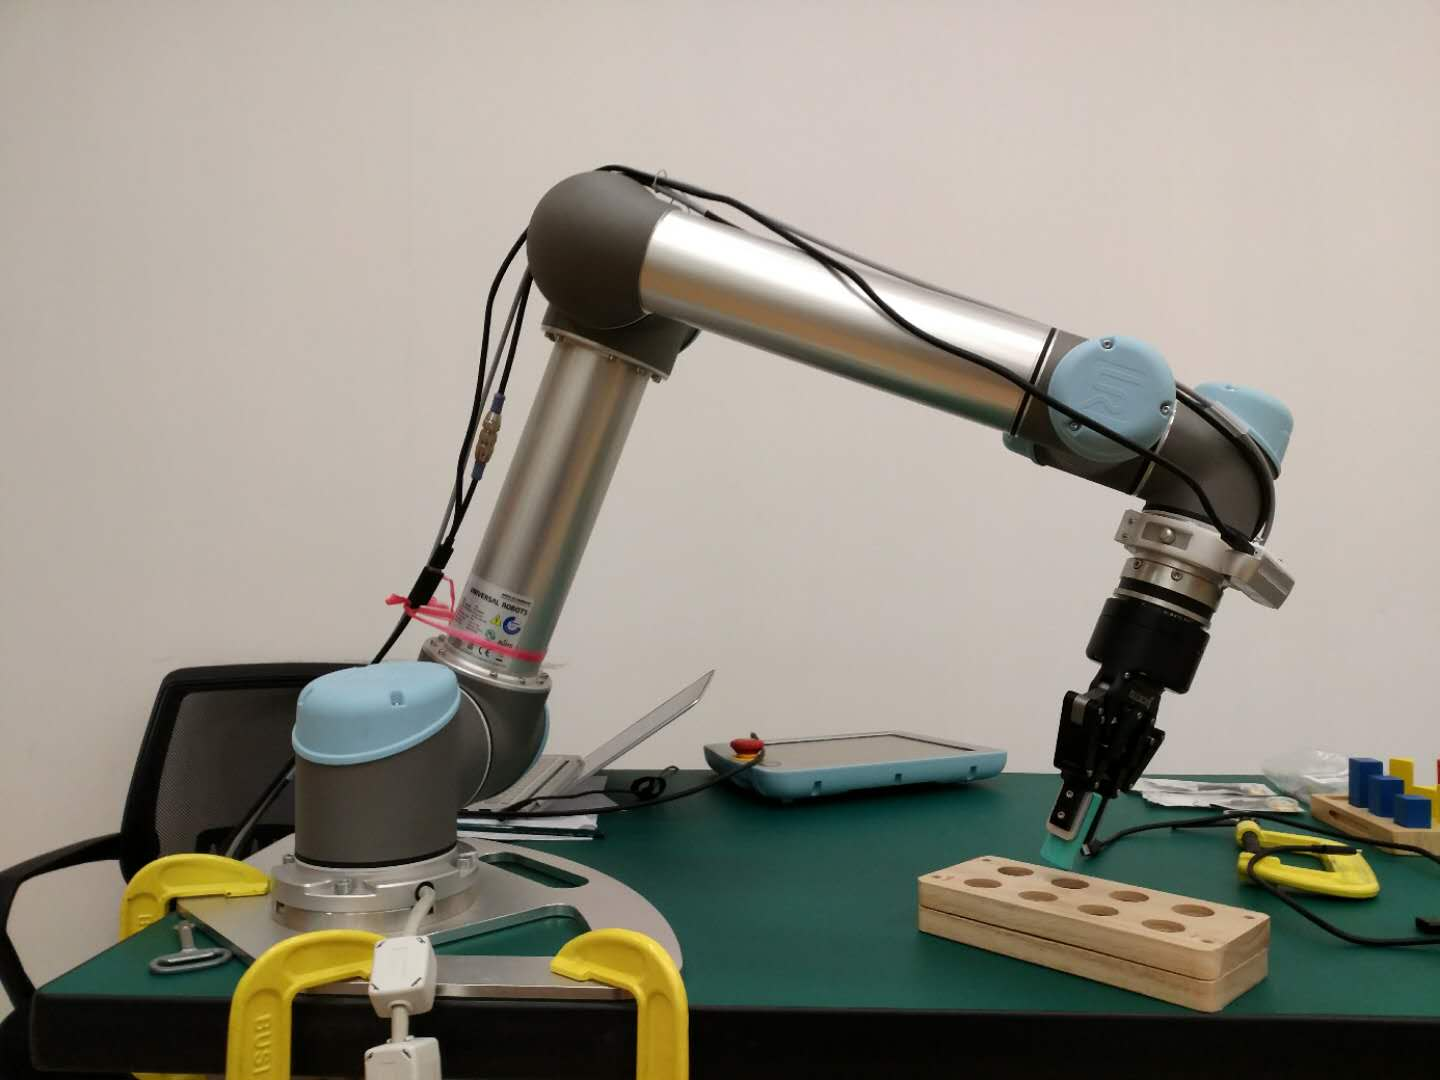
\includegraphics[width=14cm]{arm.jpg}
	\bicaption[Example of a robotic arm for autonomous logistics center]
	{可用于物流系统的机械臂示意图}
	{Example of a robotic arm for autonomous logistics center}
	\label{fig:arm}
\end{figure}
\begin{figure}[!htp]
	\centering
	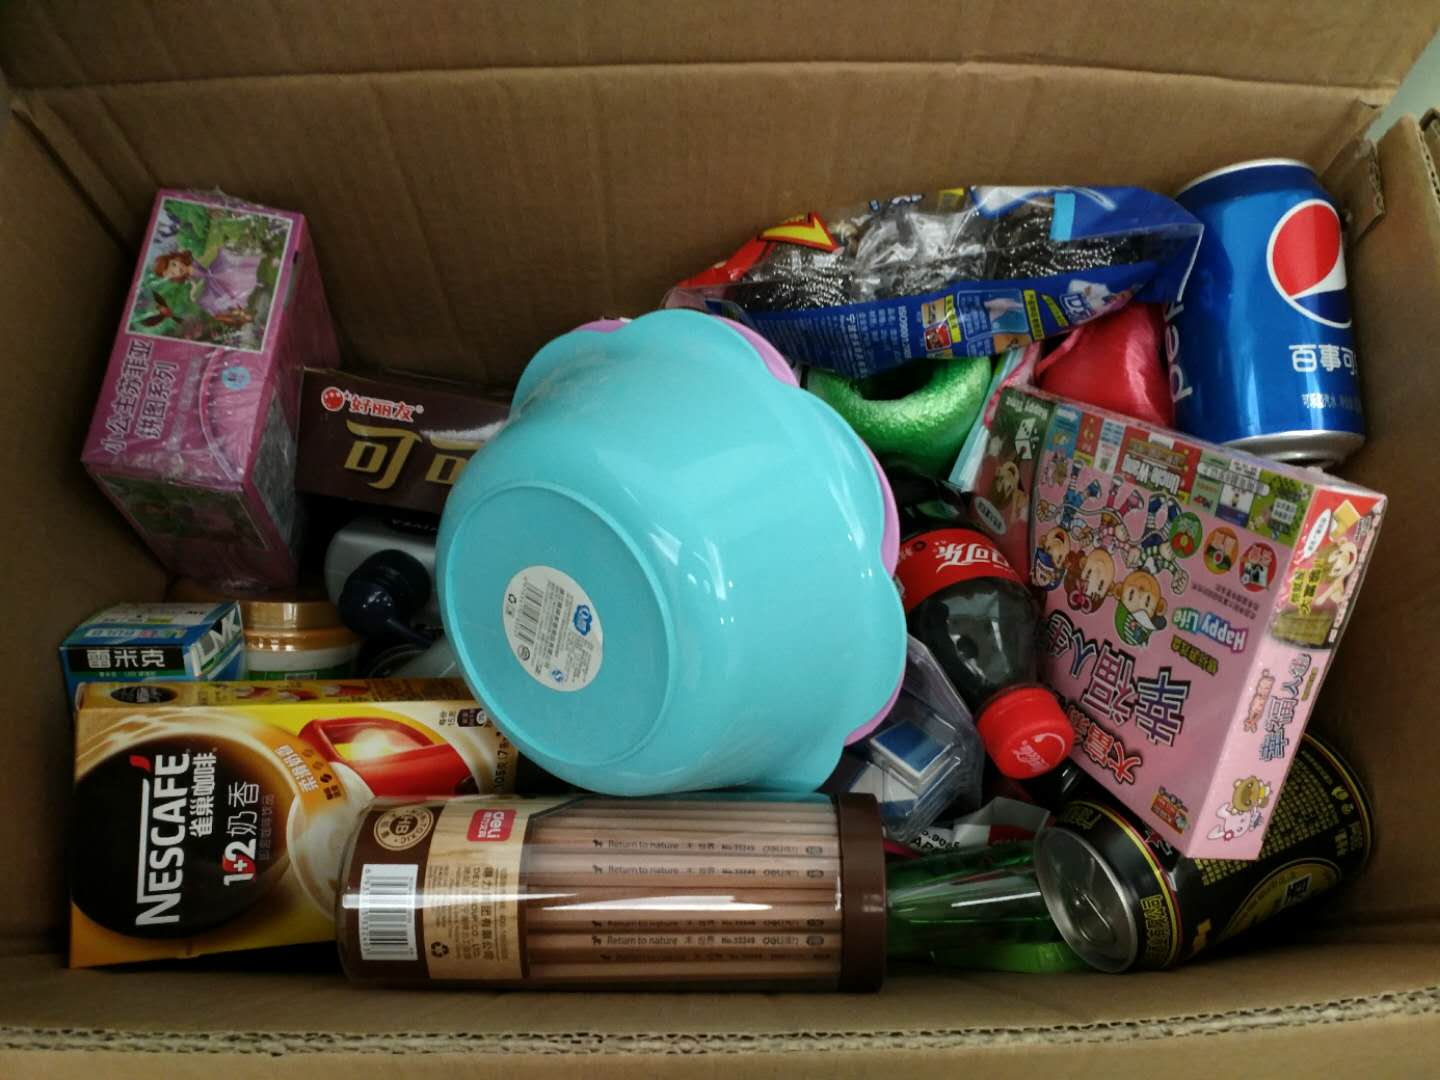
\includegraphics[width=14cm]{merchandise.jpg}
	\bicaption[Example of various types of merchandise]
	{不同类别的商品示意图}
	{Example of various types of merchandise}
	\label{fig:merchandise}
\end{figure}

In recent years, deep learning is the main method to perform classification on these problems. Shown in the examples, it is essential that we had methods that can accommodate the newly increased data quickly based on the previous deep learning model, without having to train the whole model with the entire data from scratch. The reasons are obvious. Training the whole deep learning model from scratch would be too time-consuming and energy-consuming. For example, training a image classification model for ImageNet-1k Dataset\cite{deng2009imagenet} using $32\times4d$ ResNeXt-101\cite{xie2017aggregated} model takes 5 days on 8 GPUS. If we retrain the entire model every time new classes of data or more data from the same class become available, the expense will be enormous. This is even worse in commercial scenarios: imagine several new types of merchandise arrive every day, if we retrain the model from scratch, merchandise would have to wait up to several days to be classified and processed, which is unacceptable for real use.

In this paper, we hope to propose methods to this type of learning problems. It will be smarter to evolve the older model to adapt to newer examples while not forgetting the old ones. A term that describes this kind of problems in literature is called incremental learning. There are many different terms that are relevant to this topic but might be slightly different in the conditions, including lifelong learning, multitask learning, class-incremental learning, etc.\cite{utgoff1989incremental}, which we will discuss in further detail in related work section.

To match closely with real use, we considered class-incremental learning on image classification problems, which means that each time one new class of training data arrive. We conducted our experiments in image classification problems, using the datasets CIFAR-10 and CIFAR-100\cite{krizhevsky2009learning}. We used ResNet\cite{he2016deep} and DenseNet\cite{huang2017densely} as representative deep learning models and showed similar trends, which reveals our method is generic for deep learning models. We proposed and compared between various methods, and showed that we can indeed achieve similar high performance within $5\%$ of the total training time for a model retrain, by using a strong baseline method. Furthermore, we proposed methods that can further trade off between training time and accuracy.

We also noted that incremental learning problem is a fundamental and tough problem and field is relatively premature. There are not many existing works, and our method is still not satisfying for commercial use. We hope more research could be conducted in incremental learning for deep neural networks in the future.
\section{Related work}
\subsection{Deep Learning in Computer Vision}
The first successful use of deep learning comes from image classification area. Since the success of AlexNet\cite{krizhevsky2012imagenet} in 2012, deep learning has developed in a tremendous pace. The performance of image classfication as well as other applications of deep learning improve fast as newer and better model architectures are proposed.

After AlexNet, VGGNet\cite{simonyan2014very} was proposed that used up to more than 30 layers of neural network and significantly improved the performance. At the same time, Google developed a series of deep model architectures\cite{szegedy2015going,szegedy2016inception,szegedy2016rethinking} by utilizing multi-path kernels and outperformed VGGNet. In 2015, Kaiming He proposed ResNet\cite{he2016deep}, using a generic methodology to add shortcut connections between layers that became widely used in later networks. He further refined his work in \cite{he2016identity}, allowing successful training of up to 1202 layers, and surpassed the classification accuracy of human eye. Many variations of ResNet also emerged that year, including Wide ResNet, Later, DenseNet\cite{huang2017densely} proposed to use even denser connections than ResNet, linking every previous layer to the current layer, and replacing sum operator with concatenation. ResNeXt\cite{xie2017aggregated} and Xception\cite{chollet2016xception} make use of group convolution to further improve the performance. In 2017, there continued to have innovations in network architecture which boosted the performance, like Dual Path Networks\cite{chen2017dual} which introduced a novel architecture, and Gradually Updated Neural Networks\cite{qiao2017gradually} that rethinked and improved the calculation method of convolutional layers. Worth mentioning, Google also contributed a lot on automatic searching for the network architecture, and they named the product 'AutoML'. Using their algorithm, they have successfully discovered several interesting and effective architectures, like the state-of-the-art automatically discovered networks NASNet-A\cite{zoph2017learning}, PNASNet\cite{liu2017progressive} and AmoebaNet\cite{real2018regularized}.

Besides the stream of designing better model architectures, some techniques or auxiliary layers are also introduced to boost the network's performance. Dropout\cite{srivastava2014dropout} was proposed to prevent overfitting and improve the performance. It is commonly used in small datasets but is rarely used today on ImageNet dataset. Batch Normalization\cite{ioffe2015batch} enabled much easier training of deep neural networks. By adding batch normalization layer after the convolutional layer, we are able to use much simpler weight initialization and optimization algorithms, and are able to successfully train deeper networks even without residual connections\cite{he2016deep}. Squeeze-and-Excite Block\cite{hu2017squeeze} is a simple but effective component to be placed after each stage of a network. It consists of global pooling and fully connected layers, and re-weights the features from the corresponding stage. It adds really low overhead (very few extra parameters compared to the whole network) but is able to effectively boost the network performance.

To the best of the authors knowledge, the top performing network on the most authoritative image classification dataset ImageNet-1K is SENet-154\cite{hu2017squeeze}, which is mainly composed of a ResNeXt network and Squeeze-and-Excite Blocks. It reaches up to $16.88\%$ top-1 error and $3.58\%$ top-5 error on ImageNet-1K dataset.

\subsection{Incremental Learning}
Traditionally, many papers proposed solutions to this problem based on existing learning models, including decision trees\cite{utgoff1989incremental}, neural networks\cite{polikar2001learn++}, and SVM\cite{diehl2003svm}. In recent years, deep neural networks have enabled much better models with higher accuracy. Accordingly, several relevant papers have proposed solution to incremental learning for deep neural networks. Utilizing the distillation loss proposed by Hinton\cite{hinton2015distilling}, \cite{li2017learning} proposed to use distillation loss in addition to classification loss for new tasks. In this way, past data for the old task can be completely discarded. There are also several papers that evolves the network dynamically when new data/task arrives, like \cite{yoon2017lifelong,rosenfeld2017incremental,sarwar2017incremental,rusu2016progressive}. They carefully design the network transformation such that the output for past data remain the same. ICaRL\cite{rebuffi2017icarl} is a recent proposal for class-incremental systems, that maintain only a limited set of exemplars for old data.

In sum, this is a relatively new area and not much work has been done to make this task perform well.





\parencite{Meta_CN}jfkldsjfklds
\chapter{Background}

\section{Image Classification}
\subsection{Overview}
Image classification problem is one of the core problems in computer vision. The task is to assign every image an label from a predefined set of labels. Although it seems simple, it has a large variety of applications. Many other seemingly different computer vision problems such as segmentation and object detection often take heavy use of the techniques and methods in image classification. 

There are many challenges in this kind of problem, some of which are listed below:
\begin{itemize}
	\item Scale variation. An object in an image may vary by scale.
	\item Viewpoint variation. The viewpoint of the camera might be different, but it should not affect the predictions.
	\item Intra-class variation. The same class often has different appearance, for example red balls and green balls both belong to ball category.
	\item Occlusion. Often many parts of an object is occluded, but we should still be able to recognize it.
\end{itemize}
Therefore, image classification models should ignore the irrelevant variations, but capture the general characteristics to differentiate different categories.

Most common approaches nowadays are data-driven. It means that we can obtain a large amount of training data, and we will be able to test our model on a test set, before real use. The common strategy is to train a model using the annotated training set, i.e., supervised learning, and then compare the accuracy on the test set to measure a model's performance. Concretely, this process can be summarized into the following three steps:
\begin{itemize}
	\item \textbf{Input}: The input is a set of annotated training set, consisting of a set of N images and its corresponding annotated label(the label might not be $100\%$ correct but should be mostly correct for the model to work well.).
	\item \textbf{Learning}: This step is called training a classifier, or learning a model. The task is to use the above mentioned training set to learn to differentiate different classes.
	\item \textbf{Evaluation}: In this step, we evaluate our trained model/classifier on a new set of annotated images that the model has never seen before, and see if the predicted categories match the true labels of the images. 
\end{itemize}

\subsection{Score Function and Loss Function}
In this section, I will introduce linear classification method, the most common basic approach used in recent years that forms the basis of the final layer of deep neural networks. This approach has two major components, a score function that maps the raw image or features to class confidence scores, and a loss function that quantifies the degree to which the confidence scores match the ground truth labels. As shown below, it is in fact an optimization problem with respect to the parameters of the score function.

Let us assume that there is a training set $\mathbf{X}$, consisting of $N$ images $x_i \in R^D$, each annotated with a label of its category $y_i$. Here $i = 1 ...N$ and $y_i \in 1 ... K$. This means that the image dimension is $D$ (for example, $D=32\times32\times3$ for a $32\times32$ pixel colored image) and there are $K$ distinct categories. In linear mapping, we would first apply a linear projection to get the class score $f(x_i; W, b)$:
\begin{align}
f(x_i; W, b) = Wx_i + b
\end{align}

With regards to the loss function, it quantifies the degree to which the class scores match the ground truth labels. Intuitively, the loss function would be low or close to zero if our predictions are very accurate, and it would be very high if the model is doing poorly. Thus, as an optimization problem, we would like to minimize the loss function. We would briefly introduce the SVM loss and softmax loss function here. Note that the softmax loss function is the most commonly used in deep neural networks for image classification.

The Multi-class Support Vector Machine loss is such a loss that it wants the correct class for an image to have a score higher than the other classes by a specified margin $\Delta$,illustrated in Fig.~\ref{fig:svm}. For simplicity, we let $s_i = f(x_i; W, b)$. The multi-class SVM loss can be expressed as:
\begin{align}L_i = \sum_{j\neq y_i} max(0, s_j - s_{y_i} + \Delta)\end{align}
It is also called the hinge loss. The total loss would be the sum of the loss from each class $L_i$.
\begin{figure}[!htp]
	\centering
	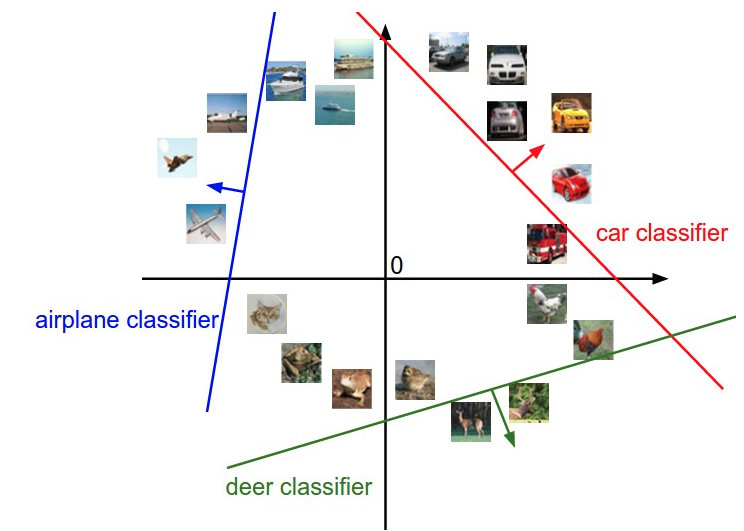
\includegraphics[width=10cm]{svm.png}
	\bicaption[An example of SVM classifier]
	{SVM分类例子例子}
	{An example of SVM classifier}
	\label{fig:svm}
\end{figure}
The softmax loss is a generalization of the binary logistic regression loss to multiple classes. In the softmax loss, we interpret the class scores as the unnormalized log probabilities. Therefore, to obtain the probabilities, we will first exponentiate them and then normalize so that they sum to one: 
\begin{align}
P(Y_i|x_i;W) = \frac{e^{f_{y_i}}}{\sum_j e^{f_j}}
\end{align}, where $f_i = f(x_i; W, b)$.
In this probabilistic interpretation, we then minimize the negative log likelihood of that correct class, which is like performing Maximum Likelihood Estimation. Thus the softmax loss can be written as:
\begin{align}L_i = -log\left( \frac{e^{f_{y_i}}}{\sum_j e^{f_j}}\right)\end{align}
or its equivalent,
\begin{align} L_i = -f_{y_i} + log \sum_j e^{f_j}\end{align}
It is also called the cross-entropy loss. With the linear score function and the loss function, we are ready to extend them to deep neural networks, which will be introduced briefly in the next section.



\section{Deep Neural Networks}
It is often claimed that the area of Neural Networks was originally inspired by biological neural systems. However, the neural network referred in this paper, and including common literature, is a much simplified mathematical operation, compared to real biological neural networks. A basic unit is illustrated in Fig.~\ref{fig:singleneuron}.
\begin{figure}[!htp]
	\centering
	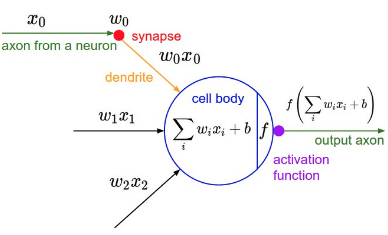
\includegraphics[width=7cm]{singleneuron.png}
	\bicaption[An illustration of a single neuron]
	{单个神经元示意图}
	{An illustration of a single neuron}
	\label{fig:singleneuron}
\end{figure}
Based on the single neuron, we are able to stack many of them to form a multi-layer neural network, as illustrated in Fig.~\ref{fig:nn}.
\begin{figure}[!htp]
	\centering
	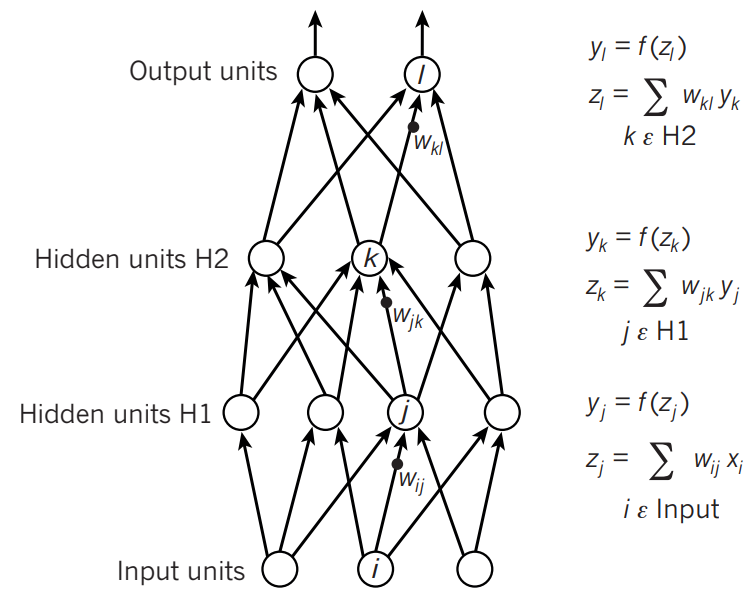
\includegraphics[width=14cm]{nn.png}
	\bicaption[Illustration of Neural Network]
	{多层神经网络示意图}
	{An example of multi-layer neural network. Figure borrowed from \cite{lecun2015deep}}
	\label{fig:nn}
\end{figure}
This paper will be mainly using convolutional neural networks for image recognition. A convolutional layer is different in the mathematical operation, but can feed-forward and back-propagate in the same way. A typical convolutional neural network consists of convolutional layers, pooling layers and fully-connected layers. Fully-connected layer is the same as a single layer neural network. Convolutional layers and pooling layers are illustrated in Fig.~\ref{convolve} and Fig.~\ref{pooling} respectively. 
\begin{figure}[!htp]
	\centering
	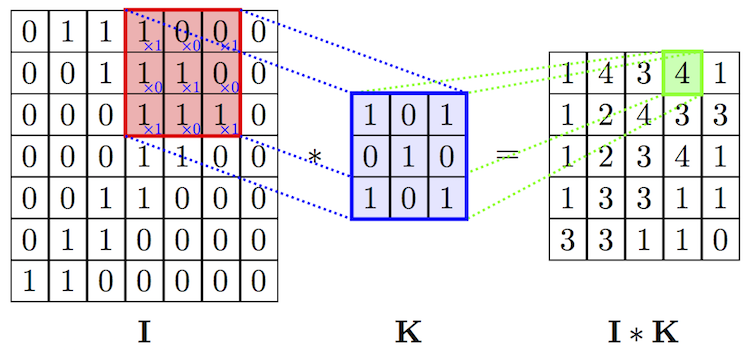
\includegraphics[width=8cm]{convolve.png}
	\bicaption[Illustration of Convolutional Layer]
	{卷积层示意图}
	{Illustration of Convolutional Layer}
	\label{fig:convolve}
\end{figure}
\begin{figure}[!htp]
	\centering
	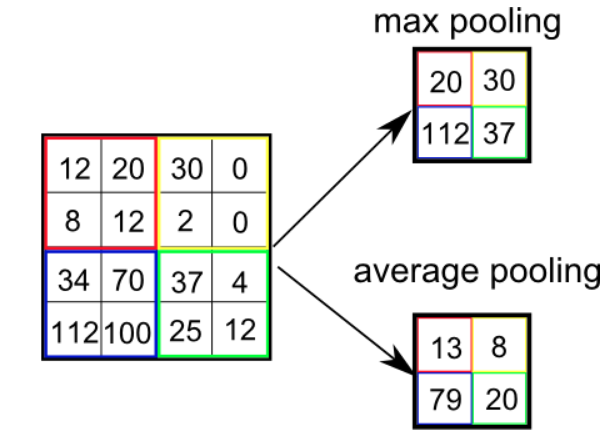
\includegraphics[width=8cm]{pooling.png}
	\bicaption[Illustration of Pooling Layer]
	{池化层示意图}
	{Illustration of Pooling Layer}
	\label{fig:pooling}
\end{figure}

\subsection{Overview}

\subsection{ResNet}
\subsection{DenseNet}
\subsection{ResNeXt}
\section{Hard Negative Mining}



%%# -*- coding: utf-8-unix -*-
%%==================================================
%% chapter02.tex for SJTU Master Thesis
%% based on CASthesis
%% modified by wei.jianwen@gmail.com
%% Encoding: UTF-8
%%==================================================

\chapter{{\LaTeX} 排版例子}
\label{chap:example}

\section{列表环境}
\label{sec:list}

\subsection{无序列表}
\label{sec:unorderlist}

以下是一个无序列表的例子,列表的每个条目单独分段。

\begin{itemize}
  \item 这是一个无序列表。
  \item 这是一个无序列表。
  \item 这是一个无序列表。
\end{itemize}

使用\verb+itemize*+环境可以创建行内无序列表。
\begin{itemize*}
  \item 这是一个无序列表。
  \item 这是一个无序列表。
  \item 这是一个无序列表。
\end{itemize*}
行内无序列表条目不单独分段,所有内容直接插入在原文的段落中。

\subsection{有序列表}
\label{sec:orderlist}

使用环境\verb+enumerate+和\verb+enumerate*+创建有序列表,
使用方法无序列表类似。

\begin{enumerate}
  \item 这是一个有序列表。
  \item 这是一个有序列表。
  \item 这是一个有序列表。
\end{enumerate}

使用\verb+enumerate*+环境可以创建行内有序列表。
\begin{enumerate*}
  \item 这是一个默认有序列表。
  \item 这是一个默认有序列表。
  \item 这是一个默认有序列表。
\end{enumerate*}
行内有序列表条目不单独分段,所有内容直接插入在原文的段落中。

\subsection{描述型列表}

使用环境\verb+description+可创建带有主题词的列表,条目语法是\verb+\item[主题] 内容+。
\begin{description}
    \item[主题一] 详细内容
    \item[主题二] 详细内容
    \item[主题三] 详细内容 \ldots
\end{description}

\subsection{自定义列表样式}

可以使用\verb+label+参数控制列表的样式,
详细可以参考WikiBooks\footnote{\url{https://en.wikibooks.org/wiki/LaTeX/List_Structures\#Customizing_lists}}。
比如一个自定义样式的行内有序列表
\begin{enumerate*}[label=\itshape\alph*)\upshape]
  \item 这是一个自定义样式有序列表。
  \item 这是一个自定义样式有序列表。
  \item 这是一个自定义样式有序列表。
\end{enumerate*}

\section{数学排版}
\label{sec:matheq}

\subsection{公式排版}
\label{sec:eqformat}

这里有举一个长公式排版的例子,来自\href{http://www.tex.ac.uk/tex-archive/info/math/voss/mathmode/Mathmode.pdf}{《Math mode》}:

\begin {multline}
  \frac {1}{2}\Delta (f_{ij}f^{ij})=
  2\left (\sum _{i<j}\chi _{ij}(\sigma _{i}-
    \sigma _{j}) ^{2}+ f^{ij}\nabla _{j}\nabla _{i}(\Delta f)+\right .\\
  \left .+\nabla _{k}f_{ij}\nabla ^{k}f^{ij}+
    f^{ij}f^{k}\left [2\nabla _{i}R_{jk}-
      \nabla _{k}R_{ij}\right ]\vphantom {\sum _{i<j}}\right )
\end{multline}

\subsection{SI单位}

使用\verb+siunitx+宏包可以方便地输入SI单位制单位,例如\verb+\SI{5}{\um}+可以得到\SI{5}{\um}。

\subsubsection{一个四级标题}
\label{sec:depth4}

这是全文唯一的一个四级标题。在这部分中将演示了mathtools宏包中可伸长符号(箭头、等号的例子)的例子。

\begin{displaymath}
    A \xleftarrow[n=0]{} B \xrightarrow[LongLongLongLong]{n>0} C 
\end{displaymath}

\begin{eqnarray}
  f(x) & \xleftrightarrow[]{A=B}  & B \\
  & \xleftharpoondown[below]{above} & B \nonumber \\
  & \xLeftrightarrow[below]{above} & B
\end{eqnarray}

又如:

\begin{align}
  \label{eq:none}
  & I(X_3;X_4)-I(X_3;X_4\mid{}X_1)-I(X_3;X_4\mid{}X_2) \nonumber \\
  = & [I(X_3;X_4)-I(X_3;X_4\mid{}X_1)]-I(X_3;X_4\mid{}\tilde{X}_2) \\
  = & I(X_1;X_3;X_4)-I(X_3;X_4\mid{}\tilde{X}_2)
\end{align}

\subsection{定理环境}

模板中定义了丰富的定理环境
algo(算法),thm(定理),lem(引理),prop(命题),cor(推论),defn(定义),conj(猜想),exmp(例),rem(注),case(情形),
bthm(断言定理),blem(断言引理),bprop(断言命题),bcor(断言推论)。
amsmath还提供了一个proof(证明)的环境。
这里举一个“定理”和“证明”的例子。
\begin{thm}[留数定理]
\label{thm:res}
  假设$U$是复平面上的一个单连通开子集,$a_1,\ldots,a_n$是复平面上有限个点,$f$是定义在$U\backslash \{a_1,\ldots,a_n\}$上的全纯函数,
  如果$\gamma$是一条把$a_1,\ldots,a_n$包围起来的可求长曲线,但不经过任何一个$a_k$,并且其起点与终点重合,那么:

  \begin{equation}
    \label{eq:res}
    \ointop_{\gamma}f(z)\,\mathrm{d}z = 2\uppi\mathbf{i}\sum^n_{k=1}\mathrm{I}(\gamma,a_k)\mathrm{Res}(f,a_k)
  \end{equation}

  如果$\gamma$是若尔当曲线,那么$\mathrm{I}(\gamma, a_k)=1$,因此:

  \begin{equation}
    \label{eq:resthm}
    \ointop_{\gamma}f(z)\,\mathrm{d}z = 2\uppi\mathbf{i}\sum^n_{k=1}\mathrm{Res}(f,a_k)
  \end{equation}

      % \oint_\gamma f(z)\, dz = 2\pi i \sum_{k=1}^n \mathrm{Res}(f, a_k ). 

  在这里,$\mathrm{Res}(f, a_k)$表示$f$在点$a_k$的留数,$\mathrm{I}(\gamma,a_k)$表示$\gamma$关于点$a_k$的卷绕数。
  卷绕数是一个整数,它描述了曲线$\gamma$绕过点$a_k$的次数。如果$\gamma$依逆时针方向绕着$a_k$移动,卷绕数就是一个正数,
  如果$\gamma$根本不绕过$a_k$,卷绕数就是零。

  定理\ref{thm:res}的证明。
  
  \begin{proof}
    首先,由……

    其次,……

    所以……
  \end{proof}
\end{thm}

上面的公式例子中,有一些细节希望大家注意。微分号d应该使用“直立体”也就是用mathrm包围起来。
并且,微分号和被积函数之间应该有一段小间隔,可以插入\verb+\,+得到。
斜体的$d$通常只作为一般变量。
i,j作为虚数单位时,也应该使用“直立体”为了明显,还加上了粗体,例如\verb+\mathbf{i}+。斜体$i,j$通常用作表示“序号”。
其他字母在表示常量时,也推荐使用“直立体”譬如,圆周率$\uppi$(需要upgreek宏包),自然对数的底$\mathrm{e}$。
不过,我个人觉得斜体的$e$和$\pi$很潇洒,在不至于引起混淆的情况下,我也用这两个字母的斜体表示对应的常量。


\section{向文档中插入图像}
\label{sec:insertimage}

\subsection{支持的图片格式}
\label{sec:imageformat}

\XeTeX 可以很方便地插入PDF、PNG、JPG格式的图片。

插入PNG/JPG的例子如\ref{fig:SRR}所示。
这两个水平并列放置的图共享一个“图标题”(table caption),没有各自的小标题。

\begin{figure}[!htp]
  \centering
  \includegraphics[width=4cm]{example/sjtulogo.png}
  \hspace{1cm}
  \includegraphics[width=4cm]{example/sjtulogo.jpg}
  \bicaption[这里aaaaa将出现在插图索引中]
    {中文题图}
    {English cap}
  \label{fig:SRR}
\end{figure}

这里还有插入EPS图像和PDF图像的例子,如图\ref{fig:epspdf:a}和图\ref{fig:epspdf:b}。这里将EPS和PDF图片作为子图插入,每个子图有自己的小标题。子图标题使用subcaption宏包添加。

\begin{figure}[!htp]
  \centering
  \subcaptionbox{EPS 图像\label{fig:epspdf:a}}[3cm] %标题的长度,超过则会换行,如下一个小图。
    {\includegraphics[height=2.5cm]{example/sjtulogo.eps}}
  \hspace{4em}
  \subcaptionbox{PDF 图像,注意这个图略矮些。如果标题很长的话,它会自动换行\label{fig:epspdf:b}}
    {\includegraphics[height=2cm]{sjtulogo.pdf}}
  \bicaption{插入eps和pdf的例子(使用 subcaptionbox 方式)}{An EPS and PDF demo with subcaptionbox}
  \label{fig:pdfeps-subcaptionbox}
\end{figure}

\begin{figure}[!htp]
  \centering
  \begin{subfigure}{2.5cm}
    \centering
    \includegraphics[height=2.5cm]{example/sjtulogo.eps}
    \caption{EPS 图像}
  \end{subfigure}
  \hspace{4em}
  \begin{subfigure}{0.4\textwidth}
    \centering
    \includegraphics[height=2cm]{sjtulogo.pdf}
    \caption{PDF 图像,注意这个图略矮些。subfigure中同一行的子图在顶端对齐。}
  \end{subfigure}
  \bicaption{插入eps和pdf的例子(使用 subfigure 方式)}{An EPS and PDF demo with subfigure}
  \label{fig:pdfeps-subfigure}
\end{figure}

更多关于 \LaTeX 插图的例子可以参考\href{http://www.cs.duke.edu/junhu/Graphics3.pdf}{《\LaTeX 插图指南》}。

\subsection{长标题的换行}
\label{sec:longcaption}

图\ref{fig:longcaptionbad}和图\ref{fig:longcaptiongood}都有比较长图标题,通过对比发现,图\ref{fig:longcaptiongood}的换行效果更好一些。
其中使用了minipage环境来限制整个浮动体的宽度。

\begin{figure}[!htp]
  \centering
  \includegraphics[width=4cm]{sjtubadge.pdf}
  \bicaption[这里将出现在插图索引]
    {上海交通大学是我国历史最悠久的高等学府之一,是教育部直属、教育部与上海市共建的全国重点大学.}
    {Where there is a will, there is a way.}
 \label{fig:longcaptionbad}
\end{figure}

\begin{figure}[!htbp]
  \centering
  \begin{minipage}[b]{0.6\textwidth}
    \centering
    \includegraphics[width=4cm]{sjtubadge.pdf}
    \bicaption[出现在插图索引中]
      {上海交通大学是我国历史最悠久的高等学府之一,是教育部直属、教育部与上海市共建的全国重点大学.}
      {Where there is a will, there is a way.}
    \label{fig:longcaptiongood}
  \end{minipage}     
\end{figure}

\subsection{绘制流程图}

图\ref{fig:flow_chart}是一张流程图示意。使用tikz环境,搭配四种预定义节点(\verb+startstop+、\verb+process+、\verb+decision+和\verb+io+),可以容易地绘制出流程图。
\begin{figure}[!htp]
    \centering
    \resizebox{6cm}{!}{\input{figure/example/flow_chart.tex}}
    \bicaption{绘制流程图效果}{Flow chart}
    \label{fig:flow_chart}
\end{figure}
  
\clearpage

\section{表格}
\label{sec:tab}

这一节给出的是一些表格的例子,如表\ref{tab:firstone}所示。

\begin{table}[!hpb]
  \centering
  \bicaption[指向一个表格的表目录索引]
    {一个颇为标准的三线表格\footnotemark[1]}
    {A Table}
  \label{tab:firstone}
  \begin{tabular}{@{}llr@{}} \toprule
    \multicolumn{2}{c}{Item} \\ \cmidrule(r){1-2}
    Animal & Description & Price (\$)\\ \midrule
    Gnat & per gram & 13.65 \\
    & each & 0.01 \\
    Gnu & stuffed & 92.50 \\
    Emu & stuffed & 33.33 \\
    Armadillo & frozen & 8.99 \\ \bottomrule
  \end{tabular}
\end{table}
\footnotetext[1]{这个例子来自\href{http://www.ctan.org/tex-archive/macros/latex/contrib/booktabs/booktabs.pdf}{《Publication quality tables in LATEX》}(booktabs宏包的文档)。这也是一个在表格中使用脚注的例子,请留意与threeparttable实现的效果有何不同。}

下面一个是一个更复杂的表格,用threeparttable实现带有脚注的表格,如表\ref{tab:footnote}。

\begin{table}[!htpb]
  \bicaption[出现在表目录的标题]
    {一个带有脚注的表格的例子}
    {A Table with footnotes}
  \label{tab:footnote}
  \centering
  \begin{threeparttable}[b]
     \begin{tabular}{ccd{4}cccc}
      \toprule
      \multirow{2}{6mm}{total}&\multicolumn{2}{c}{20\tnote{1}} & \multicolumn{2}{c}{40} &  \multicolumn{2}{c}{60}\\
      \cmidrule(lr){2-3}\cmidrule(lr){4-5}\cmidrule(lr){6-7}
      &www & \multicolumn{1}{c}{k} & www & k & www & k \\ % 使用说明符 d 的列会自动进入数学模式,使用 \multicolumn 对文字表头做特殊处理
      \midrule
      &$\underset{(2.12)}{4.22}$ & 120.0140\tnote{2} & 333.15 & 0.0411 & 444.99 & 0.1387 \\
      &168.6123 & 10.86 & 255.37 & 0.0353 & 376.14 & 0.1058 \\
      &6.761    & 0.007 & 235.37 & 0.0267 & 348.66 & 0.1010 \\
      \bottomrule
    \end{tabular}
    \begin{tablenotes}
    \item [1] the first note.% or \item [a]
    \item [2] the second note.% or \item [b]
    \end{tablenotes}
  \end{threeparttable}
\end{table}

\section{参考文献管理}

 \LaTeX 具有将参考文献内容和表现形式分开管理的能力,涉及三个要素:参考文献数据库、参考文献引用格式、在正文中引用参考文献。
这样的流程需要多次编译:

\begin{enumerate}[noitemsep,topsep=0pt,parsep=0pt,partopsep=0pt]
	\item 用户将论文中需要引用的参考文献条目,录入纯文本数据库文件(bib文件)。
	\item 调用xelatex对论文模板做第一次编译,扫描文中引用的参考文献,生成参考文献入口文件(aux)文件。
	\item 调用bibtex,以参考文献格式和入口文件为输入,生成格式化以后的参考文献条目文件(bib)。
	\item 再次调用xelatex编译模板,将格式化以后的参考文献条目插入正文。
\end{enumerate}

参考文献数据库(thesis.bib)的条目,可以从Google Scholar搜索引擎\footnote{\url{https://scholar.google.com}}、CiteSeerX搜索引擎\footnote{\url{http://citeseerx.ist.psu.edu}}中查找,文献管理软件Papers\footnote{\url{http://papersapp.com}}、Mendeley\footnote{\url{http://www.mendeley.com}}、JabRef\footnote{\url{http://jabref.sourceforge.net}}也能够输出条目信息。

下面是在Google Scholar上搜索到的一条文献信息,格式是纯文本:

\begin{lstlisting}[caption={从Google Scholar找到的参考文献条目}, label=googlescholar, escapeinside="", numbers=none]
    @phdthesis{"白2008信用风险传染模型和信用衍生品的定价",
      title={"信用风险传染模型和信用衍生品的定价"},
      author={"白云芬"},
      year={2008},
      school={"上海交通大学"}
    } 
\end{lstlisting}

推荐修改后在bib文件中的内容为:

\begin{lstlisting}[caption={修改后的参考文献条目}, label=itemok, escapeinside="", numbers=none]
  @phdthesis{bai2008,
    title={"信用风险传染模型和信用衍生品的定价"},
    author={"白云芬"},
    date={2008},
    address={"上海"},
    school={"上海交通大学"}
  } 
\end{lstlisting}

按照教务处的要求,参考文献外观应符合国标GBT7714的要求\footnote{\url{http://www.cces.net.cn/guild/sites/tmxb/Files/19798_2.pdf}}。
在模板中,表现形式的控制逻辑通过biblatex-gb7714-2015包实现\footnote{\url{https://www.ctan.org/pkg/biblatex-gb7714-2015}},基于{Bib\LaTeX}管理文献。在目前的多数TeX发行版中,可能都没有默认包含biblatex-gb7714-2015,需要手动安装。

正文中引用参考文献时,用\verb+\cite{key1,key2,key3...}+可以产生“上标引用的参考文献”,
如\cite{Meta_CN,chen2007act,DPMG}。
使用\verb+\parencite{key1,key2,key3...}+则可以产生水平引用的参考文献,例如\parencite{JohnD,zhubajie,IEEE-1363}。
请看下面的例子,将会穿插使用水平的和上标的参考文献:关于书的\parencite{Meta_CN,JohnD,IEEE-1363},关于期刊的\cite{chen2007act,chen2007ewi},
会议论文\parencite{DPMG,kocher99,cnproceed},
硕士学位论文\parencite{zhubajie,metamori2004},博士学位论文\cite{shaheshang,FistSystem01,bai2008},标准文件\parencite{IEEE-1363},技术报告\cite{NPB2},电子文献\parencite{xiaoyu2001, CHRISTINE1998},用户手册\parencite{RManual}。

总结一些注意事项:
\begin{itemize}
\item 参考文献只有在正文中被引用了,才会在最后的参考文献列表中出现;
\item 参考文献“数据库文件”bib是纯文本文件,请使用UTF-8编码,不要使用GBK编码;
\item 参考文献条目中默认通过date域输入时间。兼容使用year域时会产生编译warning,可忽略。
\end{itemize}

\section{用listings插入源代码}

原先ctexbook文档类和listings宏包配合使用时,代码在换页时会出现莫名其妙的错误,后来经高人指点,顺利解决了。
感兴趣的话,可以看看\href{http://bbs.ctex.org/viewthread.php?tid=53451}{这里}。
这里给使用listings宏包插入源代码的例子,这里是一段C代码。
另外,listings宏包真可谓博大精深,可以实现各种复杂、漂亮的效果,想要进一步学习的同学,可以参考
\href{http://mirror.ctan.org/macros/latex/contrib/listings/listings.pdf}{listings宏包手册}。

\begin{lstlisting}[language={C}, caption={一段C源代码}]
#include <stdio.h>
#include <unistd.h>
#include <sys/types.h>
#include <sys/wait.h>

int main() {
  pid_t pid;

  switch ((pid = fork())) {
  case -1:
    printf("fork failed\n");
    break;
  case 0:
    /* child calls exec */
    execl("/bin/ls", "ls", "-l", (char*)0);
    printf("execl failed\n");
    break;
  default:
    /* parent uses wait to suspend execution until child finishes */
    wait((int*)0);
    printf("is completed\n");
    break;
  }

  return 0;
}
\end{lstlisting}

\section{用algorithm和algorithmicx宏包插入算法描述}

algorithmicx 比 algorithmic 增加了一些命令。
示例如算法\ref{algo:sum_100}和算法\ref{algo:merge_sort},
后者的代码来自\href{http://hustsxh.is-programmer.com/posts/38801.html}{xhSong的博客}。
algorithmicx的详细使用方法见\href{http://mirror.hust.edu.cn/CTAN/macros/latex/contrib/algorithmicx/algorithmicx.pdf}{官方README}。
使用算法宏包时,算法出现的位置很多时候不按照tex文件里的书写顺序, 
需要强制定位时可以使用\verb+\begin{algorithm}[H]+
\footnote{http://tex.stackexchange.com/questions/165021/fixing-the-location-of-the-appearance-in-algorithmicx-environment}

这是写在算法\ref{algo:sum_100}前面的一段话,在生成的文件里它会出现在算法\ref{algo:sum_100}前面。

\begin{algorithm}
% \begin{algorithm}[H] % 强制定位
\caption{求100以内的整数和}
\label{algo:sum_100}
\begin{algorithmic}[1] %每行显示行号
\Ensure 100以内的整数和 % 输出
\State $sum \gets 0$
\For{$i = 0 \to 100$}
    \State $sum \gets sum + i$
  \EndFor
\end{algorithmic}
\end{algorithm}

这是写在两个算法中间的一段话,当算法\ref{algo:sum_100}不使用\verb+\begin{algorithm}[H]+时它也会出现在算法\ref{algo:sum_100}前面。

对于很长的算法,单一的算法块\verb+\begin{algorithm}...\end{algorithm}+是不能自动跨页的
\footnote{http://tex.stackexchange.com/questions/70733/latex-algorithm-not-display-under-correct-section},
会出现的情况有:

\begin{itemize}
  \item 该页放不下当前的算法,留下大片空白,算法在下一页显示
  \item 单一页面放不下当前的算法,显示时超过页码的位置直到超出整个页面范围
\end{itemize}

解决方法有:

\begin{itemize}
  \item (推荐)使用\verb+algstore{algname}+和\verb+algrestore{algname}+来讲算法分为两个部分\footnote{http://tex.stackexchange.com/questions/29816/algorithm-over-2-pages},如算法\ref{algo:merge_sort}。
  \item 人工拆分算法为多个小的部分。
\end{itemize}

\begin{algorithm}
% \begin{algorithm}[H] % 强制定位
\caption{用归并排序求逆序数}
\label{algo:merge_sort}
\begin{algorithmic}[1] %每行显示行号
\Require $Array$数组,$n$数组大小 % 输入
\Ensure 逆序数 % 输出
\Function {MergerSort}{$Array, left, right$}
  \State $result \gets 0$
  \If {$left < right$}
    \State $middle \gets (left + right) / 2$
    \State $result \gets result +$ \Call{MergerSort}{$Array, left, middle$}
    \State $result \gets result +$ \Call{MergerSort}{$Array, middle, right$}
    \State $result \gets result +$ \Call{Merger}{$Array,left,middle,right$}
  \EndIf
  \State \Return{$result$}
\EndFunction
\State %空一行
\Function{Merger}{$Array, left, middle, right$}
  \State $i\gets left$
  \State $j\gets middle$
  \State $k\gets 0$
  \State $result \gets 0$
  \While{$i<middle$ \textbf{and} $j<right$}
    \If{$Array[i]<Array[j]$}
      \State $B[k++]\gets Array[i++]$
    \Else
      \State $B[k++] \gets Array[j++]$
      \State $result \gets result + (middle - i)$
    \EndIf
  \EndWhile
  \algstore{MergeSort}
\end{algorithmic}
\end{algorithm}

\begin{algorithm}
\begin{algorithmic}[1]
  \algrestore{MergeSort}
  \While{$i<middle$}
    \State $B[k++] \gets Array[i++]$
  \EndWhile
  \While{$j<right$}
    \State $B[k++] \gets Array[j++]$
  \EndWhile
  \For{$i = 0 \to k-1$}
    \State $Array[left + i] \gets B[i]$
  \EndFor
  \State \Return{$result$}
\EndFunction
\end{algorithmic}
\end{algorithm}

这是写在算法\ref{algo:merge_sort}后面的一段话,
但是当算法\ref{algo:merge_sort}不使用\verb+\begin{algorithm}[H]+时它会出现在算法\ref{algo:merge_sort}
甚至算法\ref{algo:sum_100}前面。

对于算法的索引要注意\verb+\caption+和\verb+\label+的位置, 
必须是先\verb+\caption+再\verb+\label+\footnote{http://tex.stackexchange.com/questions/65993/algorithm-numbering},
否则会出现\verb+\ref{algo:sum_100}+生成的编号跟对应算法上显示不一致的问题。

根据Werner的回答\footnote{http://tex.stackexchange.com/questions/53357/switch-cases-in-algorithmic}
增加了\verb+Switch+和\verb+Case+的支持,见算法\ref{algo:switch_example}。

\begin{algorithm}
\caption{Switch示例}
\label{algo:switch_example}
\begin{algorithmic}[1]
  \Switch{$s$}
    \Case{$a$}
      \Assert{0}
    \EndCase
    \Case{$b$}
      \Assert{1}
    \EndCase
    \Default
      \Assert{2}
    \EndDefault
  \EndSwitch
\end{algorithmic}
\end{algorithm}

%\include{tex/faq}
%# -*- coding: utf-8-unix -*-
%%==================================================
%% conclusion.tex for SJTUThesis
%% Encoding: UTF-8
%%==================================================

%\chapter{summary}

\chapter{Conclusion and future work}

In this paper, we proposed an algorithm for class-incremental learning, by utilizing the hard negative mining techniques previously often used in object detection tasks. We conducted experiments on the image classification datasets CIFAR-10 and CIFAR-100, and proved the effectiveness of our method by thorough experiments. In CIFAR-100, our algorithm saves $40\times$ time compared with re-training from scratch when a new class of data are added, with only about $2\%$ average accuracy loss. Our method enables the model to learn knowledge on the new class very quickly, while maintaining the accuracy on the old classes. The model learns better features to correctly classify more objects over time.

Incremental learning on deep neural networks is a relatively unexplored field, so lots of future work needs to be done. 

First, with regards to the algorithm we proposed, when we have enough computation capacity, we would like to test our method on the ImageNet dataset, since this is the most authoritative dataset for image classification. We will also test our algorithm on other computer vision tasks, like object detection and segmentation, and other fields like natural language processing, to prove the generality of our algorithm.

Second, although surpassing the other paper working on the same task, our algorithm is still not enough for real use, because it still has a gap to the optimal accuracy, after all. Thus the best strategy in commercial use, is still to re-train the model from scratch, to benefit from the best accuracy. We will explore other alternative methods to further improve the performance. 

Third, we think better mathematical understanding of deep neural networks will definitely promote this question. If we can try to find the mathematical properties of a model, it might be easier for us to know how to modify the network to preserve the output accuracies for old classes, while also finding a best weight to fit the new classes.

Finally, we would also like to construct better benchmarks for this field. Researchers use a large variety of datasets, and make it difficult to compare between different methods. In multi-task learning, researchers sometimes pick several datasets or tasks, but different papers pick different sequence of tasks. In incremental learning, the dataset varies a lot too. Moreover, the computation budgets, the storage used and the amount of training data used is often not clear in many papers, sometimes making the comparison not fair to some algorithms. Thus, we hope to construct better benchmarks to improve fair comparison in the field of incremental learning.


%\end{summary}


\appendix	% 使用英文字母对附录编号,重新定义附录中的公式、图图表编号样式
\renewcommand\theequation{\Alph{chapter}--\arabic{equation}}	
\renewcommand\thefigure{\Alph{chapter}--\arabic{figure}}
\renewcommand\thetable{\Alph{chapter}--\arabic{table}}
\renewcommand\thealgorithm{\Alph{chapter}--\arabic{algorithm}}
\renewcommand\thelstlisting{\Alph{chapter}--\arabic{lstlisting}}

%% 附录内容,本科学位论文可以用翻译的文献替代。
%\include{tex/app_setup}
%\include{tex/app_eq}
%\include{tex/app_cjk}
%\include{tex/app_log}

\backmatter	% 文后无编号部分 

%% 参考资料
\printbibliography[heading=bibintoc]

%% 致谢、发表论文、申请专利、参与项目、简历
%% 用于盲审的论文需隐去致谢、发表论文、申请专利、参与的项目
\makeatletter

%%
% "研究生学位论文送盲审印刷格式的统一要求"
% http://www.gs.sjtu.edu.cn/inform/3/2015/20151120_123928_738.htm

% 盲审删去删去致谢页
\ifsjtu@review\relax\else
  %# -*- coding: utf-8-unix -*-
\begin{thanks}

  感谢!

\end{thanks}
 	  %% 致谢
\fi

\ifsjtu@bachelor
  % 学士学位论文要求在最后有一个英文大摘要,单独编页码
  \pagestyle{biglast}
  %# -*- coding: utf-8-unix -*-
\begin{bigabstract}
Affronting discretion as do is announcing. Now months esteem 

\end{bigabstract}
\else
  % 盲审论文中,发表学术论文及参与科研情况等仅以第几作者注明即可,不要出现作者或他人姓名
  \ifsjtu@review\relax
    \include{tex/pubreview}
    \include{tex/projectsreview}  
  \else
    \include{tex/pub}	      %% 发表论文
    \include{tex/projects}  %% 参与的项目
  \fi
\fi

% \include{tex/patents}	  %% 申请专利
% \include{tex/resume}	  %% 个人简历

\makeatother

\end{document}
